\section{Results}\label{section:results}
\par{
	Although the proposed architecture was not fully implemented, both the \emph{detector} and the \emph{classificator} were proven effective. Indeed, the concept proof of the described defect detection system on steel surfaces was proven by the results reported in \emph{Section \ref{section:results:detector}} and \emph{Section \ref{section:results:classificator}}.
}
\par{
	From results in \emph{Section \ref{section:results:classificator}} one can infer that the proposed novel usage of the dilatation factor in the first convolutional layer may represents an effective alternative to cropping when dealing with images of different sizes.
}

\subsection{Detector}\label{section:results:detector}
\par{
	The Bayesian optimization was performed using batches of $128$ images and $50$ iterations. During each iteration, the average loss function was computed over the batch and used to predict the next point in the hyperparameters domain. 
%	Losses of $0.78$, $0.92$, $0.68$ and $0.59$ were obtained with detectors of classes $1$, $2$, $3$ and $4$ respectively.
}
\par{
	After the optimization procedure, the trained detectors were tested using batches of $1024$ images ($720$ for the class $3$) and computing on them the accuracy measure:
	\begin{equation*}
	\mathcal{A} = \frac{\lvert X \cap Y \rvert}{\lvert Y \rvert}.
	\end{equation*}
}
\begin{table}
	\centering
	\normalsize	
	\begin{tabular}{|c|c|c|c|c|c|}
		\hline		
		\textbf{No.} & \textbf{Equal.} & \textbf{MinMax} & \textbf{Batch} & \textbf{Loss} & \textbf{Accuracy}\\ \hline
		\multirow{3}{*}{1} & no & no & 1024 & 0.8773 & 0.6234 \\
		& no & yes & 1024 & \textbf{0.8378} & \textbf{0.5477} \\
		& yes & no & 1024 & 0.9205 & 0.6752 \\
		& yes & yes & 1024 & 0.7977 & 0.4925 \\ \hline
		\multirow{3}{*}{2} & no & no & 760 & 0.9103 & 0.7318\\
		& no & yes & 760 & \textbf{0.9061} & \textbf{0.7738} \\
		& yes & no & 760 & 0.9676 & 0.9587 \\
		& yes & yes & 760 & 0.9172 & 0.3333 \\ \hline
		\multirow{3}{*}{3} & no & no & 1024 & 0.7382 & 0.6710 \\
		& no & yes & 1024 & \textbf{0.6852} & \textbf{0.6168} \\
		& yes & no & 1024 & 0.8161 & 0.9145 \\
		& yes & yes & 1024 & 0.6995 & 0.4600 \\ \hline
		\multirow{3}{*}{4} & no & no & 1024 & 0.6261 & 0.6190 \\
		& no & yes & 1024 & \textbf{0.6455} & \textbf{0.7528} \\
		& yes & no & 1024 & 0.6694 & 0.7334 \\
		& yes & yes & 1024 & 0.6050 & 0.5550 \\ \hline
	\end{tabular}
	\vspace{0.25cm}
	\caption{Comparison between performances obtained by different class (No.) detectors, either using or not the equalization and the MinMax normalization. In bold are reported the best detectors obtained, according to the study.}\label{table:test-bayesopt}
\end{table}
\par{
	In \emph{Table \ref{table:test-bayesopt}} are reported the average loss and accuracy obtained by the trained detectors, either using or not the equalization and the MinMax normalization on the images. These results need to be studied recalling that the defects have been identified with bounding boxes. Hence, overhead pixels are intrinsically part of our approach and the values of the loss functions have a lower bound greater than $0$.
}
\par{
	At first glance, it is clear that either in the equalized and in the non-equalized setting, the MinMax normalization improves the performance of each detector. Indeed, despite the accuracy increase by using normalization, also the loss increase. This means that the localization of more defects is not due to an increase of the detector precision, but only to the introduction of more overhead pixels.
}
\begin{table}
	\centering
	\normalsize
	\begin{tabular}{|c|c|c|c|c|}
		\hline
		\textbf{Parameters} & \textbf{Class 1} & \textbf{Class 2} & \textbf{Class 3} & \textbf{Class 4}\\ \hline
		$N$ & 4 & 3 & 3 & 3 \\ \hline
		$U$ & 11 & 7 & 16 & 15 \\ \hline
		$\lambda$ & 4.2905 & 4.0612 & 4.5523 & 3.9422 \\ \hline
		$s$ & 1.7205 & 2.3772 & 2.9674 & 2.8169 \\ \hline
		$T_{low}$ & 43 & 54 & 49 & 53 \\ \hline
		$T_{high}$ & 242 & 164 & 126 & 106 \\ \hline
		$\alpha$ & 12 & 13 & 12 & 19 \\ \hline
		$T_{hole}$ & 14168 & 14536 & 10651 & 10594 \\ \hline
		$T_{region}$ & 541 & 1158 & 682 & 1204 \\ \hline
	\end{tabular}
	\vspace{0.25cm}
	\caption{Optimal parameters obtained for each class with Bayesian optimization (non-equalized setting).}
	\label{table:params-bayesopt}
\end{table}
\begin{figure}
	\centering
	\includegraphics[width=\linewidth]{graphics/results/detector-result-class1-1}
	\vskip .05cm
	\includegraphics[width=\linewidth]{graphics/results/detector-result-class1-2}
	\vskip .05cm
	\includegraphics[width=\linewidth]{graphics/results/detector-result-class1-3}
	\vskip .05cm
	\includegraphics[width=\linewidth]{graphics/results/detector-result-class1-4}
	\vskip .05cm
	\caption{An example of the region proposal procedure performed on an image with a defect of class No.1.}\label{fig:detector-results-1}
\end{figure}
\begin{figure}
	\centering
	\includegraphics[width=\linewidth]{graphics/results/detector-result-class2-1}
	\vskip .05cm
	\includegraphics[width=\linewidth]{graphics/results/detector-result-class2-2}
	\vskip .05cm
	\includegraphics[width=\linewidth]{graphics/results/detector-result-class2-3}
	\vskip .05cm
	\includegraphics[width=\linewidth]{graphics/results/detector-result-class2-4}
	\vskip .05cm
	\caption{An example of the region proposal procedure performed on an image with a defect of class No.2.}\label{fig:detector-results-2}
\end{figure}
\begin{figure}
	\centering
	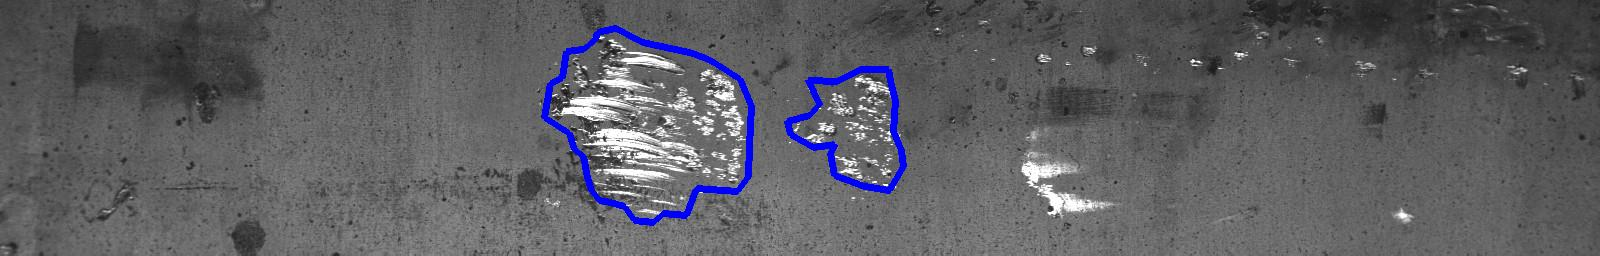
\includegraphics[width=\linewidth]{graphics/results/detector-result-class3-1}
	\vskip .05cm
	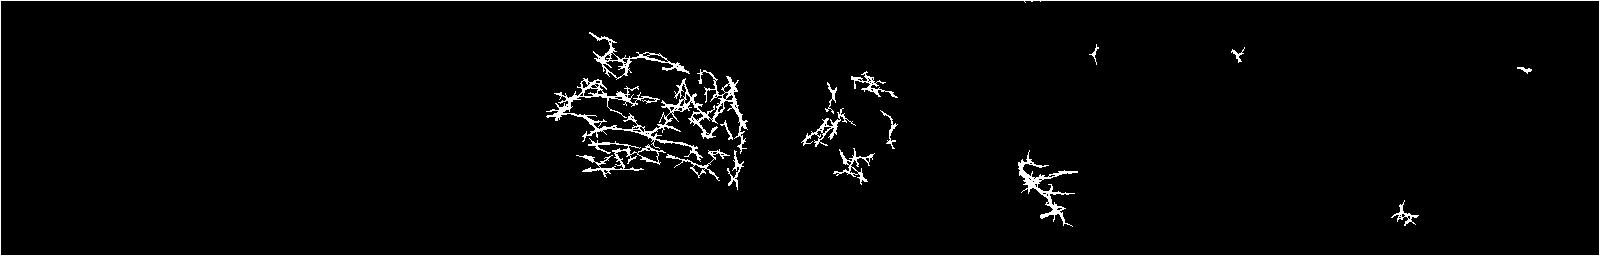
\includegraphics[width=\linewidth]{graphics/results/detector-result-class3-2}
	\vskip .05cm
	
\includegraphics[width=\linewidth]{graphics/results/detector-result-class3-3}
	\vskip .05cm
	
\includegraphics[width=\linewidth]{graphics/results/detector-result-class3-4}
	\vskip .05cm
	\caption{An example of the region proposal procedure performed on an image with a defect of class No.3.}\label{fig:detector-results-3}
\end{figure}
\begin{figure}
	\centering
	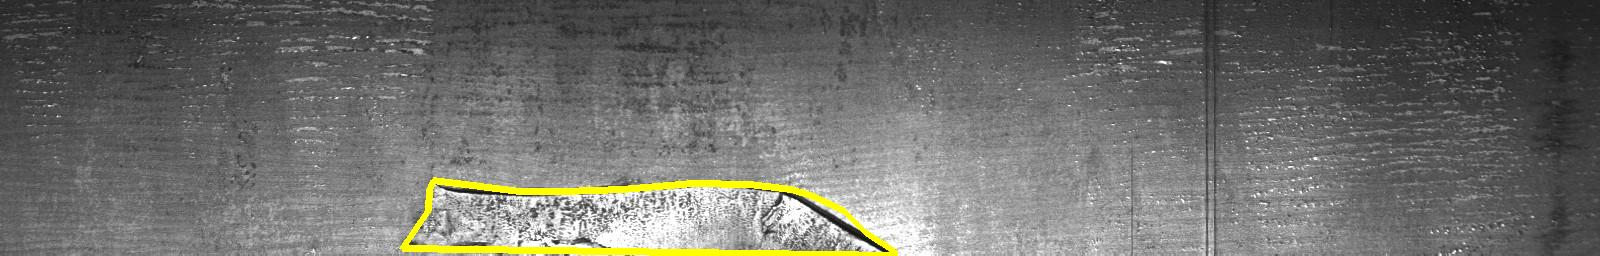
\includegraphics[width=\linewidth]{graphics/results/detector-result-class4-1}
	\vskip .05cm
	
\includegraphics[width=\linewidth]{graphics/results/detector-result-class4-2}
	\vskip .05cm
	
\includegraphics[width=\linewidth]{graphics/results/detector-result-class4-3}
	\vskip .05cm
	
\includegraphics[width=\linewidth]{graphics/results/detector-result-class4-4}
	\vskip .05cm
	\caption{An example of the region proposal procedure performed on an image with a defect of class No.4.}\label{fig:detector-results-4}
\end{figure}
\begin{figure}
	\centering
	\includegraphics[width=\linewidth]{graphics/results/acc-segmentation-class1}
	\vskip .05cm
	\includegraphics[width=\linewidth]{graphics/results/acc-segmentation-class2}
	\vskip .05cm
	\includegraphics[width=\linewidth]{graphics/results/acc-segmentation-class3}
	\vskip .05cm
	\includegraphics[width=\linewidth]{graphics/results/acc-segmentation-class4}
	\vskip .05cm
	\caption{Accuracies distributions of the trained detectors, computed on their test sets (non-equalized setting).}\label{fig:segmentation-test}
\end{figure}
\par{
	Let consider first the detectors obtained without equalization. Accuracies $0.55$, $0.77$, $0.62$ and $0.75$ have been reached for classes $1$, $2$, $3$ and $4$ respectively. Classes $3$ and $4$ have the lowest values of loss function, which means that the detection of these defects is generally more precise and with lower amount of overhead pixels.
}
\par{
	In \emph{Table \ref{table:params-bayesopt}} the optimal parameters values are reported. It is visible that tuned parameters reflect the shape of defects studied in \emph{Section \ref{subsection:defects}}. In \emph{Figure \ref{fig:detector-results-1}, \ref{fig:detector-results-2}, \ref{fig:detector-results-3}} and \emph{\ref{fig:detector-results-4}} are shown some examples of localization of defects from class $1$, $2$, $3$ and $4$ respectively. In \emph{Figure \ref{fig:segmentation-test}} the test accuracies distribution for each detector class are reported. 
}
\begin{figure}
	\centering
	\includegraphics[width=\linewidth]{graphics/results/acc-segmentation-class1-eq}
	\vskip .05cm
	\includegraphics[width=\linewidth]{graphics/results/acc-segmentation-class2-eq}
	\vskip .05cm
	\includegraphics[width=\linewidth]{graphics/results/acc-segmentation-class3-eq}
	\vskip .05cm
	\includegraphics[width=\linewidth]{graphics/results/acc-segmentation-class4-eq}
	\vskip .05cm
	\caption{Accuracies distributions of the trained detectors, computed on their test sets (equalized images).}\label{fig:segmentation-test-eq}
\end{figure}
\begin{table}
	\centering
	\normalsize
	\begin{tabular}{|c|c|c|c|c|}
		\hline
		\textbf{Parameters} & \textbf{Class 1} & \textbf{Class 2} & \textbf{Class 3} & \textbf{Class 4}\\ \hline
		$N$ & 3 & 4 & 5 & 4 \\ \hline
		$U$ & 15 & 7 & 5 & 15 \\ \hline
		$\lambda$ & 3.9199 & 2.3621 & 4.9810 & 3.5076 \\ \hline
		$s$ & 2.1161 & 1.5552 & 1.5559 & 1.4307 \\ \hline
		$T_{low}$ & 59 & 77 & 60 & 59 \\ \hline
		$T_{high}$ & 113 & 212 & 104 & 179 \\ \hline
		$\alpha$ & 7 & 8 & 6 & 6 \\ \hline
		$T_{hole}$ & 9593 & 6460 & 7179 & 9986 \\ \hline
		$T_{region}$ & 510 & 942 & 727 & 1134 \\ \hline
	\end{tabular}
	\vspace{0.25cm}
	\caption{Optimal parameters obtained for each class with Bayesian optimization (equalized setting).}
	\label{table:params-bayesopt-eq}
\end{table}
\begin{figure}
	\centering
	\includegraphics[width=\linewidth]{graphics/results/detector-result-eq-1}
	\vskip .05cm
	\includegraphics[width=\linewidth]{graphics/results/detector-result-eq-2}
	\vskip .05cm
	\includegraphics[width=\linewidth]{graphics/results/detector-result-eq-3}
	\vskip .05cm
	\includegraphics[width=\linewidth]{graphics/results/detector-result-eq-4}
	\vskip .05cm
	\includegraphics[width=\linewidth]{graphics/results/detector-result-eq-1-2}
	\vskip .05cm
	\includegraphics[width=\linewidth]{graphics/results/detector-result-eq-2-2}
	\vskip .05cm
	\includegraphics[width=\linewidth]{graphics/results/detector-result-eq-3-2}
	\vskip .05cm
	\includegraphics[width=\linewidth]{graphics/results/detector-result-eq-4-2}
	\vskip .05cm
	\caption{Effect of the equalization on the detector performance when images have very large and black regions.}\label{fig:equalization-problems}
\end{figure}
\par{
	The distribution of accuracies in the equalized setting (\emph{Figure \ref{fig:segmentation-test-eq}}) have a very different behaviour. Indeed, there is a larger amount of images with values of accuracies near zero. Hence, average accuracies of $0.49$, $0.33$, $0.46$ and $0.55$ only have been reached for classes $1$, $2$, $3$ and $4$ respectively.
}
\par{
	One of the main problems behind this results is that a \emph{global} equalization procedure has been used. Indeed, if there are very wide and monochromatic regions (e.g., black backgrounds), not significant patterns may arise  (e.g., noise). Examples of these situations are shown in \emph{Figure \ref{fig:segmentation-test-eq}}. This have a negative impact on the optimization procedure and the optimum values of parameters obtained (\emph{Table \ref{table:params-bayesopt-eq}}).
}
\par{
	On the other hand, despite the accuracies of equalized detectors are lower, the obtained losses are slightly different from the non-equalized ones. This means that, even if a equalized detector find only few defects, the proportion of overhead pixels is lower. Hence, equalized detectors seems to be more precise. This is also confirmed by the performance of the classificator, which perform better on equalized images.
}
\par{
	These results suggest that higher performance could be obtained by detectors by using a proper equalization procedure, which is able to identify the \emph{local} presence of the situation described above.
}

\subsection{Classificator}\label{section:results:classificator}
\begin{figure}
	\centering
	\includegraphics[width=.8\linewidth]{graphics/results/spreader-net-confusion}
	\caption{Local column confusion matrix on ideal input (with spreader layer).}\label{fig:local-confusion-spreader}
\end{figure}
\par{
	The local column was trained with a batch of $1024$ images, and mini-batch size of $256$.
}
\par{
	The confusion matrix of the proposed architecture for the local column on a test set of $1000\times 4$ defects is reported in \emph{Figure \ref{fig:local-confusion-spreader}}. It is visible that the defect class No. 3 is the most misclassified. This situation is probably due to the aggregation of multiple defects into the same defective region. Hence, the variability of the local features hamper the network learning.
}
\begin{figure}
	\centering
	\includegraphics[width=.8\linewidth]{graphics/results/crop-net-confusion}
	\caption{Local column confusion matrix on ideal input (with crop).}\label{fig:local-confusion-crop}
\end{figure}
\par{
	To evaluate the effectivenes of the spreader layer, a CNN with the same layers but without the novel layer was trained and tested with the same training options, i.e. batch size of $1024$, mini-batch size of $256$ and $30$ epochs. An optimal learning rate was used for both. In \emph{Figure \ref{fig:local-confusion-crop}} its confusion matrix is illustrated.
}
\par{
	It is interesting to notice that the network with the spreading layer achieves higher accuracy ($+0.7\%$) then the one which uses cropping instead. Moreover, the former overcome the latter in classifying defects of class No. 3 and No. 4. Indeed, these are the wider defects in the dataset. Hence, one can infer that the spreader layer deals better then cropping with larger images. This is visible also comparing the gained percentage with the outliers percentage, reported in the first row of \emph{Table \ref{table:cropping}}.
}
\par{
	However, neither one of the two CNNs overfits, and both can be trained longer. Moreover, deeper architectures can be used along with either image cropping or the spreading layer. With more powerful hardware, these could easily reach higher accuracies. 
}
\begin{figure}
	\centering
	\includegraphics[width=\linewidth]{graphics/results/spreader-net-confusion-noneq}
	\caption{Local column confusion matrix on ideal input (images non-equalized).}\label{fig:local-confusion-noneq}
\end{figure}
\par{
	Then, the proposed local column structure was trained also with non-equalized images, but with the same training options. The resulting confusion matrix is reported in \emph{Figure \ref{fig:local-confusion-noneq}}.
}
\par{
	It is visible that there is an actual improvement of $2.2\%$ in the average accuracy when using equalized images.
}
\begin{figure}
	\centering
	\includegraphics[width=\linewidth]{graphics/results/spreader-net-confusion-update}
	\caption{Local column confusion matrix on ideal input (with spreader, more epochs).}\label{fig:local-confusion-spreader-update}
\end{figure}
\par{
	Hence, the architectural choice is clear. The local column proposed was further trained, for other $40$ epochs, and reached ans accuracy of $75\%$. However, it kept the same structure, and thus the same number of parameters. It is predictable that a deeper model with a larger training set will achieve state-of-the-art results. The updated confusion matrix is illustrated in \emph{Figure \ref{fig:local-confusion-spreader-update}}.
}
\subsection{Architecture implementation}
\par{
	The whole system implementation can be found in the \href{https://github.com/antonioterpin/wavelet_ml}{\texttt{GitHub}} repository \cite{antonioterpin:github}.
}

\section{Further work}\label{section:further-work}
\par{
	This work can be further developed in many ways.
}
\subsection{Proposed architecture improvement}
\par{
	Firstly, it would be interesting to implement and train the shape column, preeptively discarding misleading data, and the global column and measure their contribution. The structure of the shape column may be identical to the local column, described in \emph{Section \ref{section:local-column}}.
}
\par{
	Regarding the local column, some padding could be considered around defective regions, to fed the CNN also with some more pixels outside the border.
}
\par{
	Secondly, the final classifier should be implemented to realize the end-to-end system and evaluate its performance.
}
\par{
	Thirdly, as announced in \emph{Section \ref{section:local-column}}, both the local and the shape column could be fed with a cropped image. One could attempt to preemptively discard these outliers and try to optimize the other samples with a smaller input and, hence, more traditional classificators.
}
\begin{table*}
	\centering
	\normalsize
	\begin{tabular}{|c|c|c|c|c|c|}
		\hline
		\textbf{Cropping size} & \textbf{Class No.1 outliers} & \textbf{Class No.2 outliers}& \textbf{Class No.3 outliers} & \textbf{Class No.4 outliers} & \textbf{Overall outliers}\\\hline
		$800\times 800$ & $0\%$ & $0\%$ & $1.47\%$ & $1.06\%$ & $0.88\%$\\
		$512\times 512$ & $0\%$ & $0\%$ & $2.94\%$ & $3.99\%$ & $2.11\%$\\
		$256\times 256$ & $0\%$ & $0\%$ & $6.61\%$ & $17.57\%$& $6.42\%$\\
		\hline
	\end{tabular}
	\vspace{0.5cm}
	\caption{Cropping examples.}\label{table:cropping}
\end{table*}
\par{
	Some examples of interesting cropping size are shown in \emph{Table \ref{table:cropping}}.
}
\subsection{Challenger}
\par{
	Some comparisons with a challenger architecture are needed to evaluate the effectiveness of the proposed system.
}
\par{
	As an example, a well-known \emph{sliding window} classificator could be used.
}
\subsubsection{Sliding window architecture}
\par{
	The idea behind this architecture is to crop the input image at different locations (eventually all the ones possible, as in this paper) and use a classifier to assign to the pixels of the considered region an array of confidences.
}
\begin{figure}
	\centering
	\includegraphics[width=\linewidth]{graphics/results/detector-problem-1}
	\vskip .05cm
	\includegraphics[width=\linewidth]{graphics/results/detector-problem-2}
	\vskip .05cm
	\includegraphics[width=\linewidth]{graphics/results/detector-problem-3}
	\vskip .05cm
	\includegraphics[width=\linewidth]{graphics/results/detector-problem-4}
	\vskip .05cm
	\caption{COMMENTARE PROBLEMI}\label{fig:detector-problems}
\end{figure}
\begin{figure}
	\centering
	\begin{tikzpicture}
	% Image
	\node[rectangle, draw, minimum width=3cm, minimum height=3cm] (image) at (0,0) {Image};
	% Window
	\node[rectangle, draw=red, minimum width=.8cm, minimum height=.8cm] (window) at ($(image) + (.3,.9)$) {};
	% Sliding window
	\draw[->, draw=red] ($(window) + (.2,0)$) -- ($(window) + (1,0)$);
	\draw[->, draw=red] ($(window) + (0,-.2)$) -- ($(window) + (0,-.7)$);
	% Classifier
	\node[rounded rectangle, draw, minimum width=2cm, minimum height=1cm] (classifier) at ($(image) + (2.5,0)$) {Classifier};
	\draw[->,draw=blue] ($(window) + (0,0)$) -- (classifier);
	% Confidence map
	\node[rectangle,draw,minimum width=3cm, minimum height=3cm] (confidence map) at ($(classifier) + (2.5,0)$) {Confidence map};
	\node[rectangle, draw=red, minimum width=.8cm, minimum height=.8cm] (confidence map window) at ($(confidence map) + (.3,.9)$) {};
	\draw[->, draw=red] ($(confidence map window) + (.2,0)$) -- ($(confidence map window) + (1,0)$);
	\draw[->, draw=red] ($(confidence map window) + (0,-.2)$) -- ($(confidence map window) + (0,-.7)$);
	\draw[->,draw=blue] (classifier) -- ($(confidence map window)$);
	\end{tikzpicture}
	\caption{Sliding window architecture}\label{fig:sliding-window}
\end{figure}
\par{
	This cropped regions may overlap. In those circumstances, an heuristic to combine different values of confidences is needed.
}
\par{
	In \emph{Figure \ref{fig:sliding-window}} the sketch of this architecture is shown. In the illustration the resulting map, called \emph{confidence map}, is associated to an array of confidences relative to the possible labels. 
}
\par{
	The \emph{confidence map} is then used along with some image segmentation tecnique to spot defective regions. In particular, a $n+1$ levels whatershed algorithm is proposed in \emph{Section \ref{section:challenger:image-segmentation}}.
}
\par{
	Since defects may have different dimensions, more refined tecniques could be used to improve the accuracy of the challenger. However, these are outside the scope of this work, and they are proposed as a further development in \emph{Section \ref{section:further-work}}. Moreover, the segmentation tecnique proposed in \emph{Section \ref{section:challenger:image-segmentation}} soothes this problem, since it combines local information from different areas to build the defective regions.
}
\subsubsection{Image segmentation}\label{section:challenger:image-segmentation}
\par{
	The \emph{confidence map} is used to segmentate the image through a $n+1$ levels whatershed algorithm. However, since the defective regions are always disjunct, the problem can be reduced to a binary whatershed algorithm \cite{ieee:87344} considering all the defective classes as one, and distinguishing them only later. The $n+1$ levels whatershed algorithm is left as a further development in \emph{Section \ref{section:further-work}}.
}
\par{
	As a final remark about the challenger, it is patent that even this naive implementation is far more involved then the proposed architecture, and the reason lies on the image segmentation approach.
}
\par{
	Moreover, the challenger could be further refined. As an example, a multi-scale approach could be considered, since the challenger does not take into account the variability of defects dimensions. To solve this flaw, \emph{image pyramids} could be used.
}
\par{
	Finally, an interesting development would be to investigate further a segmentation with overlapping (adjacent) regions, when there are more classes then foreground/background only. Towards this multi-level segmentation, it would be interesting to consider a non-binary whatershed-based algorithm.
}